\documentclass[11pt]{article}
\usepackage[margin=0.7in]{geometry}
\usepackage{amsmath,amssymb,mathrsfs}
\usepackage{booktabs,graphicx}\usepackage[compact]{titlesec}
\usepackage{microtype}\usepackage{xurl}
\usepackage[hidelinks]{hyperref}

\newcommand{\Ci}{\mathscr{C}^i}\newcommand{\U}{\mathcal{U}}
\newcommand{\D}[1]{\textsf{#1}}   % equation label in the dissertation [D]
\newcommand{\words}[1]{\emph{In words:} #1}
\setlength{\parindent}{0pt}
\setlength{\parskip}{4pt}

\begin{document}
\begin{center}
{\Large Thin-Sheet Error and the TAG Mass Budget}\\[3pt]
Giovanni Fereoli \quad 6 October 2026
\end{center}

Equation labels in sans serif (e.g.\ \D{z0}) refer to the dissertation~[D].
$z$ points up, $k=k_{mn}=j_{mn}/(\alpha R^*)$ is the wavenumber of mode
$(m,n)$ and $\lambda=2\pi/k$ its wavelength.

\section*{Why the error is larger than $\sigma$}
The mass is linear in the data: the fit returns
$\Delta\hat{\mathbf c}=A^+\Delta\mathbf d$ ($A^+$ the truncated-SVD inverse)
and Wahr's inversion sums it, $\Delta\hat M=\mathbf f_M^{\sf T}\Delta\hat{\mathbf c}$.
Split the data into the field the model assumes ($\mathbf d_0$: the true
$\Delta\varrho$ as a flat sheet on $z_0$), what the assumptions leave out
($\delta\mathbf d$), and noise ($\mathbf n$). Then
\begin{equation}
  \Delta\hat M-\Delta M=
  \underbrace{\mathbf f_M^{\sf T}A^+\mathbf d_0-\Delta M}_{b_{\rm basis}}
  +\underbrace{\mathbf f_M^{\sf T}A^+\delta\mathbf d}_{b_{\rm wa}+b_{\rm th}+\dots}
  +\underbrace{\mathbf f_M^{\sf T}A^+\mathbf n}_{\rm noise},
  \qquad
  \sigma^2=\mathbf f_M^{\sf T}A^+\,\Sigma_n\,A^{+\sf T}\mathbf f_M .
  \label{eq:split}
\end{equation}
The formal $\sigma$ contains only the noise. The $b_i$ are biases: they are
the same every time, so no covariance sees them. The triangle inequality bounds
the error by
\begin{equation}
  \boxed{\;|\Delta\hat M-\Delta M|\le\sigma_{\rm sys}+2\sigma,\qquad
  \sigma_{\rm sys}=\sum_i|b_i|,\qquad
  \text{report }\ \Delta\hat M\pm\sigma\,(\text{stat})\pm\sigma_{\rm sys}\,(\text{sys}).\;}
  \label{eq:budget}
\end{equation}
\words{$\sigma$ says how far the answer would move if the noise were drawn
again. A wrong assumption moves it the same way every time, so $\sigma$ cannot
see it. Each assumption adds a bias $b_i$: the estimator applied to the signal
that the assumption leaves out. The Result below gives that signal for the two
thin-sheet assumptions, wander and thickness, mode by mode
($\delta\Ci=\varepsilon_k\,\Ci$). The mass-kernel section turns every $b_i$
into one integral and bounds it; the TAG section gives the numbers.}

\section*{Result}
A column of moved material with thickness $\Delta h$ and middle at height
$\zeta$ above the sheet plane $z_0$ is returned by the thin-sheet model with
the relative error
\begin{equation}
  \boxed{\;
  \varepsilon_k=e^{k\zeta}\,S(k\Delta h)-1
  =\underbrace{k\zeta+\tfrac12(k\zeta)^2}_{\text{wander}}
  +\underbrace{\tfrac1{24}(k\Delta h)^2}_{\text{thickness}}+O(k^3),
  \qquad S(u)=\frac{\sinh(u/2)}{u/2}.\;}
  \label{eq:err}
\end{equation}
The two parts alone are
\begin{equation}
  \boxed{\;\varepsilon^{\rm wa}_k=e^{k\zeta}-1=k\zeta+\frac{(k\zeta)^2}{2}+\frac{(k\zeta)^3}{6}+\dots
  =\frac{2\pi\,\zeta}{\lambda}+\dots\;}
  \label{eq:wa}
\end{equation}
\begin{equation}
  \boxed{\;\varepsilon^{\rm th}_k=S(k\Delta h)-1
  =\frac{(k\Delta h)^2}{24}+\frac{(k\Delta h)^4}{1920}+\dots
  =\frac{1}{24}\Big(\frac{2\pi\,\Delta h}{\lambda}\Big)^2+\dots\;}
  \label{eq:th}
\end{equation}
For the total moved mass the wander cancels at first order, but only for modes
much longer than the footprint:
\begin{equation}
  \boxed{\;\varepsilon_M=\tfrac12(ks)^2+O(k^3)\quad\text{if }kR^*\ll1,\qquad
  s^2=\frac{\int\Delta\varrho\,\big(\zeta^2+\Delta h^2/12\big)\,dA}{\int\Delta\varrho\,dA}.\;}
  \label{eq:M}
\end{equation}

\section*{Proof}

\textbf{Step 1: the model.} The moved mass is a sheet of surface density
$\Delta\varrho$ on $z=z_0$, and each coefficient becomes a modal density by
Eq.~\D{sigma\_amn},
$\hat\sigma^{c}_{mn}=k\,\Ci_{mn}/(2\pi G)$.

\textbf{Step 2: one lifted sheet.} Mode $(m,n)$ of a sheet on $z_0$ fades
upward as $\U_{mn}\propto e^{-k(z-z_0)}$. The same sheet at $z_0+\zeta'$ gives
\begin{equation}
  e^{-k(z-z_0-\zeta')}=e^{k\zeta'}\,e^{-k(z-z_0)} .
\end{equation}
The height dependence $e^{-k(z-z_0)}$ is the one the model expects, so the fit
returns the coefficient of a sheet on $z_0$ that is $e^{k\zeta'}$ times
heavier: $\hat\sigma=e^{k\zeta'}\sigma$. The field height $z$ cancels.
\words{each mode is a wave that fades upward, and short waves fade fastest.
Mass placed higher is closer to the field points and looks heavier.}

\textbf{Step 3: a column is a stack of sheets.} The moved material in a column
has uniform density between $h_{\rm pre}$ and $h_{\rm post}$
(Eq.~\D{sigma\_h}): thickness $\Delta h=h_{\rm post}-h_{\rm pre}$, middle at
$\zeta=\tfrac12(h_{\rm pre}+h_{\rm post})-z_0$ (Eq.~\D{zeta}). Each slice
$d\zeta'$ carries the fraction $d\zeta'/\Delta h$ of the column and is
returned with the gain of Step~2. Adding the slices,
\begin{equation}
  G_k=\frac{1}{\Delta h}\int_{\zeta-\Delta h/2}^{\zeta+\Delta h/2}e^{k\zeta'}d\zeta'
  =\frac{e^{k(\zeta+\Delta h/2)}-e^{k(\zeta-\Delta h/2)}}{k\,\Delta h}
  =e^{k\zeta}\,\frac{e^{k\Delta h/2}-e^{-k\Delta h/2}}{k\,\Delta h}
  =e^{k\zeta}\,S(k\Delta h),
  \label{eq:G}
\end{equation}
using $e^{y}-e^{-y}=2\sinh y$ with $y=k\Delta h/2$. This is exact, and
$\varepsilon_k=G_k-1$ proves the first equality of~\eqref{eq:err}.
\words{the gain of the column is the average gain of its slices: one factor
for where its middle is (wander), one for how thick it is (thickness).}

\textbf{Step 4: expand.} With $x=k\zeta$ and $u=k\Delta h$,
\begin{align}
  e^{x}&=1+x+\frac{x^2}{2}+\frac{x^3}{6}+\dots
  \label{eq:exp}\\
  S(u)&=\frac{\tfrac u2+\tfrac{1}{3!}\big(\tfrac u2\big)^3+\tfrac{1}{5!}\big(\tfrac u2\big)^5+\dots}{u/2}
  =1+\frac{1}{6}\Big(\frac u2\Big)^2+\frac{1}{120}\Big(\frac u2\Big)^4+\dots
  =1+\frac{u^2}{24}+\frac{u^4}{1920}+\dots
  \label{eq:Sexp}
\end{align}
The second line is~\eqref{eq:th}. Multiplying the two,
\begin{equation}
  G_k=\Big(1+k\zeta+\tfrac12k^2\zeta^2+\dots\Big)\Big(1+\tfrac1{24}k^2\Delta h^2+\dots\Big)
  =1+k\zeta+\tfrac12k^2\zeta^2+\tfrac1{24}k^2\Delta h^2+O(k^3),
\end{equation}
which is~\eqref{eq:err}. The $O(k^3)$ remainder is
$\tfrac16(k\zeta)^3+\tfrac1{24}(k\zeta)(k\Delta h)^2$. \hfill$\square$

\textbf{Why $1/24$.} Expand the gain inside the integral instead,
$e^{k\zeta'}=1+k\zeta'+\tfrac12k^2\zeta'^2+\dots$, and average over the
column, which is uniform on $[\zeta-\Delta h/2,\ \zeta+\Delta h/2]$:
\begin{equation}
  \langle\zeta'\rangle=\zeta,\qquad
  \langle\zeta'^2\rangle=\frac{(\zeta+\Delta h/2)^3-(\zeta-\Delta h/2)^3}{3\,\Delta h}
  =\zeta^2+\frac{\Delta h^2}{12},
\end{equation}
\begin{equation}
  G_k=1+k\zeta+\tfrac12k^2\Big(\zeta^2+\frac{\Delta h^2}{12}\Big)+\dots,
  \qquad \tfrac12\cdot\tfrac1{12}=\tfrac1{24}.
\end{equation}
\words{$\Delta h^2/12$ is the variance of a uniform layer. The top half of the
column looks too heavy and the bottom half too light; the first-order parts
cancel, and only the always-positive second-order part survives. So thickness
is a small, second-order error that always over-estimates. The middle height
$\zeta$ enters at first order: that is the wander, and it is why the wander
condition below is much stricter.}

\textbf{Step 5: total mass.} $\Delta M$ is carried by the zonal modes $(0,n)$,
and the error of each is
$\int\Delta\varrho\,(G_k-1)\,J_0(k\rho)\,dA$. With
$G_k-1=k\zeta+\tfrac12k^2(\zeta^2+\Delta h^2/12)+O(k^3)$ and
$J_0(x)=1-\tfrac14x^2+\dots$,
\begin{equation}
  \int\Delta\varrho\,(G_k-1)J_0\,dA
  =k\!\int\!\Delta\varrho\,\zeta\,dA
  +\tfrac12k^2\!\int\!\Delta\varrho\Big(\zeta^2+\frac{\Delta h^2}{12}\Big)dA
  -\tfrac14k^3\!\int\!\Delta\varrho\,\zeta\rho^2\,dA+\dots
\end{equation}
Eq.~\D{z0} puts $z_0$ at the centroid of the signed slab: since
$\tfrac12(h_{\rm post}^2-h_{\rm pre}^2)=\Delta h\,(\zeta+z_0)$, it reads
$\sum\Delta h\,(\zeta+z_0)=z_0\sum\Delta h$, i.e.\ $\sum\Delta h\,\zeta=0$. So
$\int\Delta\varrho\,\zeta\,dA=0$ and the first term vanishes. Dividing by
$\int\Delta\varrho\,dA$ gives~\eqref{eq:M}. The third term is the wander again,
times $(k\rho)^2$: it is small only when $kR^*\ll1$. \hfill$\square$
\words{the sheet sits at the centre of mass, so for the total mass the
too-heavy high material and the too-light low material cancel. This holds only
for a mode that is flat across the footprint; a shorter mode weights the
centre and the rim differently, and the cancellation is lost.}

\section*{When the thin sheet is fine}
Ask each error in~\eqref{eq:err} to stay below a tolerance $\varepsilon$. Both
grow with $k$, so only the shortest mode needs checking,
$k_{\max}=k_{M-1,N}=2\pi/\lambda_{\min}$. The leading terms of~\eqref{eq:wa}
and~\eqref{eq:th} give
\begin{equation}
  \boxed{\;
  \underbrace{|\zeta|\le\frac{\varepsilon}{k_{\max}}=\frac{\varepsilon}{2\pi}\,\lambda_{\min}}_{\text{wander}},
  \qquad
  \underbrace{|\Delta h|\le\frac{\sqrt{24\,\varepsilon}}{k_{\max}}=\frac{\sqrt{24\,\varepsilon}}{2\pi}\,\lambda_{\min}}_{\text{thickness}}.\;}
  \label{eq:bound}
\end{equation}
With both present the two errors add. For the total mass, the first-order wander
cancels only for zonal modes longer than the footprint, $k_{0n}R^*\ll1$
(Eq.~\eqref{eq:M}).

\words{the middle of every column must sit close to the sheet plane, within
$\varepsilon/2\pi$ of the shortest wavelength (0.8\% of it for $\varepsilon=5\%$).
The column may be much thicker, up to $\sqrt{24\varepsilon}/2\pi$ of it (17\%),
because thickness is a second-order error and wander a first-order one.}

\section*{Mass kernel: the upper bound}
Feed the estimator 1~kg at a point $\mathbf x$. The data are its field
$\mathbf g(\mathbf x)$, and the answer is
\begin{equation}
  w(\mathbf x)=\mathbf h^{\sf T}\mathbf g(\mathbf x),\qquad
  \mathbf h=A^{+\sf T}\mathbf f_M .
\end{equation}
The real data are a sum of such points,
$\Delta\mathbf d=\int\mathbf g(\mathbf x)\,dm(\mathbf x)+\mathbf n$, and the
true mass counts the points over the footprint,
$\Delta M=\int1_{R^*}(\rho)\,dm$. Since $\Delta\hat M=\mathbf h^{\sf T}\Delta\mathbf d$,
\begin{equation}
  \boxed{\;\Delta\hat M-\Delta M=\int\big[w(\mathbf x)-1_{R^*}(\rho)\big]\,dm(\mathbf x)
  \;+\;\mathbf h^{\sf T}\mathbf n .\;}
  \label{eq:kernel}
\end{equation}
This is exact: no expansion, any mass distribution.
\words{$w(\mathbf x)$ is how many kg the estimator reports for each kg placed
at $\mathbf x$. A perfect estimator has $w=1$ under the footprint and $w=0$
outside. Every bias is the gap $w-1_{R^*}$, weighted by where the moved mass
really is.} Evaluating $w$ at three heights of each column splits the bias
exactly into the $b_i$ of~\eqref{eq:split}:
\begin{equation}
  b_{\rm basis}=\!\int\!\big(w_{z_0}-1_{R^*}\big)\,dm,\qquad
  b_{\rm wa}=\!\int\!\big(w_{\rm mid}-w_{z_0}\big)\,dm,\qquad
  b_{\rm th}=\!\int\!\big(w_{\rm col}-w_{\rm mid}\big)\,dm,
  \label{eq:bi}
\end{equation}
with $w$ taken on the sheet plane ($w_{z_0}$), at the column middle
($w_{\rm mid}$), and averaged over the column ($w_{\rm col}$).

\textbf{Closed form.} Suppose the fit returned the exact Fourier--Bessel
projection of the sheet, with no field-point fit and no SVD cutoff. A point
mass $m$ at radius $\rho$, in a column at $(\zeta,\Delta h)$, then gives the
zonal coefficient $a_n=m\,J_0(k_n\rho)\,G_{k_n}/N_n$ (orthogonality for $\rho$,
Eq.~\eqref{eq:G} for the height), with $k_n=k_{0n}$ and
$N_n=\int_{R_\alpha}J_0^2\,dA=\pi R_\alpha^2J_1(j_{0n})^2$, $R_\alpha=\alpha R^*$.
Wahr counts mode $n$ as $W_na_n$ with
$W_n=\int_{R^*}J_0(k_n\rho)\,dA=2\pi R^*J_1(k_nR^*)/k_n$; the modes with
$m\ge1$ integrate to zero over the footprint. Hence
\begin{equation}
  \boxed{\;w_N(\rho,\zeta,\Delta h)=\sum_{n=1}^{N}c_n\,J_0(k_n\rho)\,
  e^{k_n\zeta}\,S(k_n\Delta h),\qquad
  c_n=\frac{W_n}{N_n}=\frac{2R^*J_1(k_nR^*)}{k_nR_\alpha^2\,J_1(j_{0n})^2}.\;}
  \label{eq:wN}
\end{equation}
The $c_n$ are the Fourier--Bessel coefficients of the footprint $1_{R^*}$. So
on the sheet plane ($\zeta=\Delta h=0$), $w_N$ is the truncated series of a
step, and its error is the Gibbs error:
\begin{equation}
  \boxed{\;\big|w_N(\rho,0,0)-1_{R^*}(\rho)\big|\;\lesssim\;
  \min\Big\{\tfrac12,\ \frac{1}{\pi k_N\,|\rho-R^*|}\Big\},\;}
  \label{eq:gibbs}
\end{equation}
exactly $\tfrac12$ at the rim, a $9\%$ overshoot on either side, then a
$1/\text{distance}$ decay (checked numerically for TAG to within 20\%, worst on
the axis $\rho=0$).
\words{the three biases are the three factors of~\eqref{eq:wN}. Basis: with
$N$ zonal modes the footprint edge is drawn as a ramp of width
$\sim1/k_N$, so mass near the rim counts half and mass a few metres away
counts a few percent. This is not a thin-sheet effect. Wander and thickness:
the per-mode gains $e^{k\zeta}$ and $S(k\Delta h)$ of the Result, now inside
the sum. A gain on the short modes breaks the cancellation that makes the
sum close to $1_{R^*}$, so the wander is amplified, not averaged.}

\textbf{Each term in closed form.} \emph{Band limit (basis and outside).}
The $c_n$ make $w_N(\rho,0,0)=P_N1_{R^*}$, the projection of the footprint on
the first $N$ zonal modes. $P_N$ is symmetric, so with $\mu=\varrho\,\Delta h$
the mass per area,
\begin{equation}
  b_{\rm band}=\int\big(P_N1_{R^*}-1_{R^*}\big)\,\mu\,dA=\int_{R^*}\big(P_N\mu-\mu\big)\,dA ,
\end{equation}
the mass that smoothing the map to $N$ modes moves across the rim. Near the
rim ($k_NR^*\gg1$) the ramp of~\eqref{eq:gibbs} is the 1-D one,
$w_N-1_{R^*}\approx\pm\big(\tfrac12-\mathrm{Si}(k_N|\rho-R^*|)/\pi\big)$
(minus inside), whose integral is $1/(\pi k_N)$ on each side. Over the rim
length $2\pi R^*$:
\begin{equation}
  \boxed{\;b_{\rm in}\approx-\frac{2R^*}{k_N}\,\bar\mu_{\rm in},\qquad
  b_{\rm out}\approx+\frac{2R^*}{k_N}\,\bar\mu_{\rm out},\qquad
  \frac{b_{\rm band}}{\Delta M}\approx-\frac{2}{\pi k_NR^*}\,
  \frac{\bar\mu_{\rm in}-\bar\mu_{\rm out}}{\bar\mu_*},\;}
  \label{eq:rim}
\end{equation}
with $\bar\mu_{\rm in}$, $\bar\mu_{\rm out}$ the mean mass per area in the
rings of width $2/(\pi k_N)$ (the ramp's equivalent width) just inside and
just outside the rim, and $\bar\mu_*=\Delta M/\pi R^{*2}$. A rigorous bound
follows from Cauchy--Schwarz:
\begin{equation}
  |b_{\rm band}|\le T_N\,\big\|\bar\mu-P_N\bar\mu\big\|_2,\qquad
  T_N^2=\pi R^{*2}-\sum_{n\le N}\frac{W_n^2}{N_n}\approx\frac{2R^*}{k_N},
  \label{eq:cs}
\end{equation}
with $\bar\mu(\rho)$ the ring average of $\mu$, the only part $1_{R^*}$ sees.
\words{$N$ modes draw the rim as a ramp about $1/k_N$ wide, so they push mass
across it. The error is the jump in mass per area across the rim, times the
rim length, over $\pi k_N$. It vanishes if the rim sits where the map is flat
($\bar\mu_{\rm in}=\bar\mu_{\rm out}$), and it falls as $1/(k_NR^*)$.}

\emph{Fit (aliasing and cutoff).} With the SVD cutoff, $A^+A=VV^{\sf T}$
($V$: the kept right singular vectors). Split the field of 1~kg as
$\mathbf g(\mathbf x)=A\boldsymbol\phi(\mathbf x)+\mathbf r(\mathbf x)$, with
$\boldsymbol\phi$ the coefficients of the exact projection
($\mathbf f_M^{\sf T}\boldsymbol\phi=w_N$) and $\mathbf r$ what no mode
reproduces at the field points. Then
\begin{equation}
  w-w_N=-\mathbf f_M^{\sf T}\big(I-VV^{\sf T}\big)\boldsymbol\phi(\mathbf x)
  +\mathbf h^{\sf T}\mathbf r(\mathbf x).
\end{equation}
The first term is the part of the Wahr weights in the discarded directions
(cutoff); the second is out-of-basis field that the fit reads as CH signal
(aliasing). Both need the truth's own coefficients and field: this term has no
closed form, and only the kernel measures it.

\emph{Mesh vs point masses.} Each entry of $\mathbf g$ is a potential or a
gradient of $1/|\mathbf p-\mathbf x|$, so $w$ is harmonic in the source
position, $\nabla^2w=0$. Averaging $w$ over a cell $a\times a\times\Delta h$
changes it only at second order, by
$\tfrac{a^2}{24}\nabla_h^2w+\tfrac{\Delta h^2}{24}\partial_z^2w$, with
$\nabla_h^2w=-\partial_z^2w$:
\begin{equation}
  \boxed{\;\bar w_{\rm cell}\approx w+\frac{\Delta h^2-a^2}{24}\,\partial_z^2w,\qquad
  b_{\rm th}\approx\frac1{24}\!\int\!\Delta h^2\,\partial_z^2w\,dm,\qquad
  b_{\rm cell}\approx-\frac{a^2}{24}\!\int\!\partial_z^2w\,dm.\;}
  \label{eq:cell}
\end{equation}
Per mode $\partial_z^2=k^2$: the column gives the thickness gain
$S(k\Delta h)\approx1+(k\Delta h)^2/24$ of Eq.~\eqref{eq:Sexp}, and the cell
gives $1-(ka)^2/24$. So no mode is off by more than $(k_{\max}a)^2/24$.
\words{a cell and a point mass differ only by the cell's quadrupole. The
thickness is its vertical half, the grid spacing its horizontal half with the
opposite sign; a cube has none.}

\textbf{The bound.} Since
$\big|\int e\,dm\big|\le\int|e|\,|dm|$,~\eqref{eq:kernel} gives
\begin{equation}
  \boxed{\;|\Delta\hat M-\Delta M|\;\le\;\int\big|w-1_{R^*}\big|\,|dm|+2\sigma
  \;\le\;\max\big|w-1_{R^*}\big|\;M_{\rm moved}+2\sigma,
  \qquad M_{\rm moved}=\int|dm|.\;}
  \label{eq:anyrho}
\end{equation}
It holds for any density in the moved volume. The price is $M_{\rm moved}$:
excavated and deposited mass are added, not allowed to cancel. With the
pipeline's uniform density, $dm=\varrho\,\Delta h\,dA$, the $b_i$
of~\eqref{eq:bi} are signed and known. If the density departs from $\varrho$
by at most a fraction $\delta_\varrho$, each $dm$ moves by at most
$\delta_\varrho|dm|$, so
\begin{equation}
  \boxed{\;|\Delta\hat M-\Delta M|\;\le\;\sigma_{\rm sys}
  +\kappa\,\delta_\varrho\,|\Delta M|+2\sigma,\qquad
  \sigma_{\rm sys}=\sum_i|b_i|,\qquad
  \kappa=\frac{\int|w-1_{R^*}|\,\varrho\,|\Delta h|\,dA}{|\Delta M|}.\;}
  \label{eq:final}
\end{equation}
\words{$\kappa$ says how much each percent of density variation can move
$\Delta M$. $\delta_\varrho=0$ is the uniform-density budget~\eqref{eq:budget};
$\delta_\varrho=1$ allows any density between $0$ and $2\varrho$. Every term
is the estimator's own kernel integrated against the DTMs: no simulation, and
no knowledge of the true mass.}

\section*{TAG: error budget}
TAG basis $(\alpha;M,N)=(6;8,22)$, $R^*=8$~m: $k_{\max}=1.65$~m$^{-1}$,
$\lambda_{\min}=3.8$~m. For $\varepsilon=5\%$, Eq.~\eqref{eq:bound} asks
$|\Delta h|\le0.67$~m and $|\zeta|\le3$~cm. A typical TAG column (median over
the moved volume) has $|\Delta h|=0.36$~m and $|\zeta|=0.36$~m: the thickness
passes, the wander fails by $\times12$. So expect a negligible thickness bias
and a wander bias at the percent level.

Each $b_i$ is Eq.~\eqref{eq:bi} with the pipeline's own kernel
$w=\mathbf h^{\sf T}\mathbf g$ (same 10\,000 field points, same SVD cutoff:
64 of 352 singular values kept), evaluated at every $0.3$-m DTM column with
$dm=\varrho\,\Delta h\,dA$. Running the pipeline's fit on the field of the same
point masses gives the same numbers; the mesh row is the gap between these
point masses and the polyhedral field of the real run.
\par{\centering\small
\begin{tabular}{llrr}
\toprule
source of error & in $\sigma$? & $b_i$ (uniform $\varrho$) & bound, any $\varrho$\\
\midrule
noise & yes & $\pm0.31\%$ ($1\sigma=87$~kg) & \\
thickness, Eq.~\eqref{eq:th} & no & $-0.13\%$ & $2\%$\\
wander, Eq.~\eqref{eq:wa} & no & $+2.40\%$ & $73\%$\\
basis: band limit $+$ SVD cutoff & no & $+2.77\%$ & $54\%$\\
material outside $R^*$ & no & $+0.08\%$ & $25\%$\\
mesh vs point masses & no & $+0.19\%$ & --\\
\midrule
sum & & $+5.31\%$ & $\kappa=104\%$\\
actual error $\Delta\hat M-\Delta M$ & & $+5.30\%$ ($17\sigma$) & \\
\bottomrule
\end{tabular}\par}
\smallskip
The last column is $\int|\Delta w|\,|dm|/|\Delta M|$ for each row; $\kappa$ is
the same integral for the whole $w-1_{R^*}$, smaller than the sum of the rows.
With uniform density, Eq.~\eqref{eq:final} gives $\sigma_{\rm sys}=5.6\%$ and
\begin{equation}
  \Delta M=-2.98\times10^4~\text{kg}\ \pm87~\text{kg (stat)}\ \pm1.7\times10^3~\text{kg (sys)},
\end{equation}
which contains the true $-2.83\times10^4$~kg: $5.3\%\le5.6\%+2(0.31\%)$. A
density that varies by $\pm\delta_\varrho$ between columns adds up to
$1.04\,\delta_\varrho$: $\pm10\%$ in density allows $10\%$ more in $\Delta M$.

\textbf{Why $\kappa\approx1$.} TAG moved far more mass than it removed:
$M_{\rm moved}=7.3\,|\Delta M|$ over the patch ($4.1|\Delta M|$ excavated,
$3.2|\Delta M|$ deposited). The kernel error averaged over the moved mass is
$0.14$, and $0.14\times7.3=1.04$. Uniform density makes excavation and
deposition cancel to $5\%$; without it nothing forces them to.

\par{\centering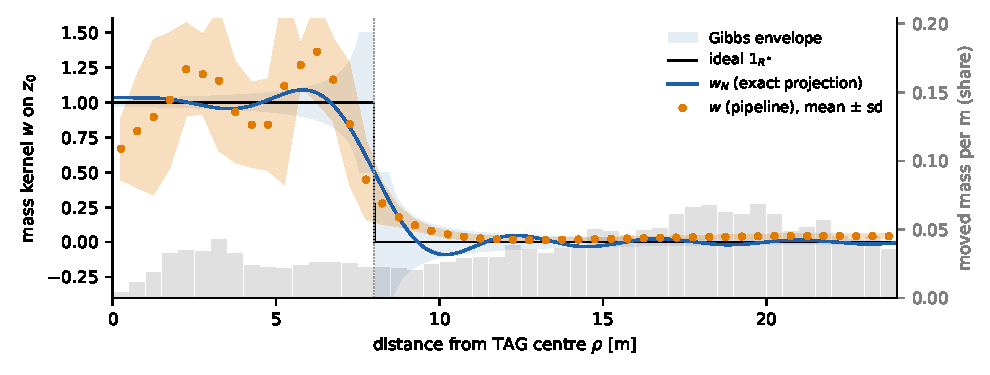
\includegraphics[width=\linewidth]{ch_thin_sheet_kernel.pdf}\par}
{\small Mass kernel on the sheet plane versus distance from the TAG centre.
Black: a perfect estimator. Blue: the closed form~\eqref{eq:wN} with the Gibbs
envelope~\eqref{eq:gibbs}. Orange: the pipeline's kernel, mean $\pm$ s.d.\ over
each 0.5-m ring of DTM columns. Grey: where the moved mass is.\par}

\textbf{The basis error.} The closed form~\eqref{eq:wN} gives the band limit
alone: $-1.94\%$ from mass inside $R^*$ and $+1.07\%$ from outside, both from
the Gibbs ramp at the rim. The pipeline gives $+2.77\%$ and $+0.08\%$. The
difference is the fit. The 352 modes cannot match the sheet's field exactly at
the field points (5\% of it is left in the residual even without noise), so
the fit bends the coefficients, the zonal ones included, to make up the rest
(aliasing). In the figure this is the $\pm0.3$--$0.5$ scatter of $w$ around
$w_N$ inside $R^*$. The SVD cutoff decides how much gets through. Without
noise:
\par{\centering\small
\begin{tabular}{lrrrr}
\toprule
SVD cutoff (values kept of 352) & $8.3\times10^{-3}$ (64) & $10^{-4}$ (119) & $10^{-6}$ (164) & $10^{-8}$ (205)\\
\midrule
$b_{\rm basis}$ & $+2.77\%$ & $+0.66\%$ & $-18.5\%$ & $+18.0\%$\\
$\sum b_i$ & $+5.1\%$ & $+1.8\%$ & $-21.6\%$ & $-34.5\%$\\
$\kappa$ & $1.04$ & $1.87$ & $2.67$ & $5.37$\\
\bottomrule
\end{tabular}\par}
\smallskip
A looser cutoff first lowers the bias, then lets aliasing through, and
$\kappa$ grows throughout. With the exact projection and all 22 zonal modes
($w_N$, no cutoff), the wander alone is $+211\%$ and $\kappa=12$: the cutoff
is what removes the large $e^{k_n\zeta}$ of the short modes. The noise-only
$\sigma$ cannot choose the cutoff; the kernel can.

\textbf{Formulas against the kernel.}
\par{\centering\small
\begin{tabular}{llrr}
\toprule
term & formula, TAG inputs & formula & exact (kernel)\\
\midrule
band limit, inside $R^*$ & Eq.~\eqref{eq:rim}, $\bar\mu_{\rm in}=0.39\,\bar\mu_*$ & $-2.18\%$ & $-1.94\%$\\
band limit, outside $R^*$ & Eq.~\eqref{eq:rim}, $\bar\mu_{\rm out}=0.22\,\bar\mu_*$ & $+1.25\%$ & $+1.07\%$\\
band limit, total & bound~\eqref{eq:cs}, $T_N=3.34$~m & $\le6.3\%$ & $-0.87\%$\\
fit: aliasing $+$ cutoff & none & -- & $+3.72\%$\\
thickness & Eq.~\eqref{eq:cell} & $-0.12\%$ & $-0.13\%$\\
cell vs point ($a=0.30$~m) & Eq.~\eqref{eq:cell} & $-0.03\%$ & \\
\bottomrule
\end{tabular}\par}
\smallskip
The rim formula is within 20\% of the exact band-limit terms. At TAG's rim
the mass per area is $0.39\,\bar\mu_*$ just inside and $0.22\,\bar\mu_*$ just
outside; the jump, $0.17\,\bar\mu_*$, times $2/(\pi k_NR^*)=0.056$ gives
$-0.9\%$. The rigorous bound~\eqref{eq:cs} is $6.3\%$ ($\bar\mu$ in rings one
grid cell wide; 18\% of its norm lies above the band). The fit, pipeline minus
exact projection ($+2.85\%-(-0.87\%)$), has no formula and is the largest part
of the basis term. The cell term is $-0.03\%$ (at most $(k_{\max}a)^2/24=1\%$
per mode); the rest of the mesh row, $+0.2\%$, is where the 0.3-m DTM height
maps and the meshes differ, a mass-map error covered by the caveat below.

\textbf{Caveats.} The $b_i$ assume uniform $\varrho$ and exact DTMs. Any error
$\delta m$ in the mass map adds at most $\int|w-1_{R^*}|\,|\delta m|$ (for a
DTM error $\delta h$, put $|\delta h|$ for $|\Delta h|$ in $\kappa$). $0.9\%$ of the
field points are within 0.5~m of the sheet, where $w$ is grainy.
$0.14\%$ of the field points lie below $z_0$ (down to $-0.21$~m). One random
draw of field points; $w$ depends on where they are.

\textbf{So:} the noise is $0.3\%$ and the systematics $5.6\%$; that is why the
error is $17\sigma$ and not $1\sigma$. Half of the systematics is the thin
sheet, almost all of it the wander, as the conditions predicted; the thickness
is $-0.1\%$. The other half is the basis, mostly the fit (aliasing and
cutoff): the band limit alone is $-0.9\%$. The analytical upper bound is
\begin{equation}
  |\Delta\hat M-\Delta M|\le5.6\%+1.04\,\delta_\varrho+0.6\%\quad\text{of }|\Delta M|,
\end{equation}
so the TAG mass is as good as the uniform-density assumption. Every $b_i$
comes from the DTMs, so it can also be removed instead of quoted: the terrain
refinement, which puts the sheet on the real surface, takes $\Delta M$ from
$+5.3\%$ to $+1.1\%$.

\vspace{4pt}
{\small [D] G.~Fereoli, \emph{Dissertation, Part~2: Cylindrical Harmonics},
\url{https://github.com/giovannifereoli/Dissertation---CH-Pt.2}.
Numbers: \path{notes/ch_thin_sheet_tag_check.py} (conditions), \path{notes/ch_thin_sheet_budget.py} (budget, kernel, bounds, figure).}
\end{document}
